\chapter{Tipos Abstractos de Datos (TADs o ADTs en inglés)}

Un tipo abstracto de datos (TAD) es una colección de valores y operaciones que se definen mediante una especificación que es independiente de cualquier representación.

Un TAD es una abstracción:
\begin{itemize}
    \item Se destacan los detalles de la especificación (el qué),
    \item Se ocultan los detalles de la implementación (el cómo).
\end{itemize}

\section{Especificación de un TAD}
Para especificar un TAD se deben definir:
\begin{enumerate}
    \item Su \textbf{nombre}.
    \item Especificar \textbf{constructores}: procedimientos o funciones mediante los cuales puedo crear elementos del tipo que estoy especificando.
    \item Especificar \textbf{operaciones}: todos los procedimientos o funciones que permitirán manipular los elementos del tipo de datos que estoy especificando.
    \item Indicamos los \textbf{tipos} de cada constructor y operación (el encabezado de los procedimientos o funciones), y mediante lenguaje natural explicamos qué hacen.
    \item Algunas operaciones pueden tener restricciones que las indicamos mediante \textbf{precondiciones}.
    \item Debemos especificar también una operación de destrucción que libera la memoria utilizada por los elementos del tipo, en caso que sea necesario.
\end{enumerate}

\subsection{Ejemplo}
Suponga que se va a desarrollar un programa para administrar la información de una biblioteca.

Puesto que allí hay elementos como ficheros, usuarios, libros, etc., que participan en el problema, en el software existirá un TAD que represente y simule la operación de cada uno de ellos: el TAD Fichero, el TAD Usuario y el TAD Libro. Estos TAD estarán relacionados dentro del programa, de la misma manera como los elementos que modelan están relacionados en la biblioteca: un elemento del TAD Usuario puede tener en préstamo un elemento del TAD Libro, los elementos del TAD Fichero tienen elementos del TAD Ficha, que representan libros de la biblioteca, etc. No existirá un TAD Pared, puesto que no participa en el problema, así haga parte de la biblioteca (a menos, claro está, que se trate de un sistema de diseño arquitectónico, en el cual las paredes sean los elementos de base.

\section{Implementación de un TAD}
\begin{itemize}
    \item Definir un nuevo tipo con el nombre del TAD especificado. Para ello utilizamos tipos concretos y otros tipos definidos previamente.
    \item Implementar cada constructor respetando los tipos tal como fueron especificados.
    \item Implementar cada operación respetando los tipos tal como fueron especificados.
    \item Implementar operación de destrucción liberando memoria si es que se ha reservado al construir los elementos.
    \item Pueden surgir nuevas restricciones que dependen de cómo implementamos el tipo.
    \item Puedo necesitar operaciones auxiliares que no están especificadas en el tipo.
\end{itemize}

\section{TAD Lista}
Las listas son colecciones 0 o mas elementos de un mismo tipo, de tamaño variable.

\subsection{Especificación}
\begin{itemize}
    \item \textbf{Nombre}: Lista
    \item \textbf{Constructores}:
    \begin{itemize}
        \item \texttt{empty()}: crea una lista vacía. 
\begin{codebox}{Constructores}
\footnotesize empty()
\tcblower
\begin{pascallike}
fun empty() ret l : List of T
{- crea una lista vacia. -}
\end{pascallike}
\end{codebox}
        \item \texttt{addl()}: agrega un elemento al comienzo de la lista.
\begin{codebox}{Constructores}
\footnotesize addl()
\tcblower
\begin{pascallike}
proc addl (in e : T, in/out l : List of T)
{- agrega el elemento e al comienzo de la lista l. -}
\end{pascallike}
\end{codebox}
    \end{itemize}
    \item \textbf{Operaciones}:
    \begin{itemize}
        \item decidir si una lista es vacía,
        \item tomar el primer elemento,
        \item tirar el primer elemento,
        \item agregar un elemento al final,
        \item obtener la cantidad de elementos,
        \item concatenar dos listas,
        \item obtener el elemento en una posición específica,
        \item tomar una cantidad arbitraria de elementos,
        \item tirar una cantidad arbitraria de elementos,
        \item copiar una lista en una nueva.
    \end{itemize}
\end{itemize}

\begin{codebox}{TAD Lista}
\begin{pascallike}
spec List of T where

constructors    
    fun empty() ret l : List of T
    {- crea una lista vacia. -}

    proc addl (in e : T, in/out l : List of T)
    {- agrega el elemento e al comienzo de la lista l. -}

destroy
    proc destroy (in/out l : List of T)
    {- Libera memoria en caso que sea necesario. -}

operations
    fun is_empty(l : List of T) ret b : bool
    {- Devuelve True si l es vacia. -}

    fun head(l : List of T) ret e : T
    {- Devuelve el primer elemento de la lista l -}

    {- PRE: not is_empty(l) -}
    proc tail(in/out l : List of T)
    {- Elimina el primer elemento de la lista l -}

    {- PRE: not is_empty(l) -}
    proc addr (in/out l : List of T,in e : T)
    {- agrega el elemento e al final de la lista l. -}

    fun length(l : List of T) ret n : nat
    {- Devuelve la cantidad de elementos de la lista l -}

    proc concat(in/out l : List of T,in l0 : List of T)
    {- Agrega al final de l todos los elementos de l0
    en el mismo orden.-}

    fun index(l : List of T,n : nat) ret e : T
    {- Devuelve el n-esimo elemento de la lista l -}

    {- PRE: length(l) > n -}
    proc take(in/out l : List of T,in n : nat)
    {- Deja en l so lo los primeros n
    elementos, eliminando el resto -}

    proc drop(in/out l : List of T,in n : nat)
    {- Elimina los primeros n elementos de l -}

    fun copy_list(l1 : List of T) ret l2 : List of T
    {- Copia todos los elementos de l1 en la nueva lista l2 -}
\end{pascallike}
\end{codebox}

\subsection{Ejempo de uso}

\begin{codebox}{Promedio}
\footnotesize Uso de operaciones de listas
\tcblower
\begin{pascallike}
fun promedio (l : List of float) ret r : float
    var largo : nat
    var elem : float
    var laux : List of float

    laux := copy(l) {- copio la lista para no modificar la original -}
    r := 0.0 {- inicializo el promedio en 0 -}
    largo := length(laux) {- obtengo la cantidad de elementos -}
    do (not is_empty(laux)) -> {- mientras la lista no sea vacia -}
        elem := head(laux) {- tomo el primer elemento -}
        r := r + elem {- sumo el elemento al promedio -}
        tail(laux) {- elimino el primer elemento -}
    od
    destroy(laux) {- libero la memoria -}
    r := r / largo {- calculo el promedio -}
end proc
\end{pascallike}
\end{codebox}

\section{Implementación de un TAD Lista mediante punteros}
\begin{itemize}
    \item Implementaremos el TAD lista utilizando punteros, implementación conocida como \texttt{lista enlazada}.
    \item Cada elemento de la lista estará alojado en un nodo conteniendo además un puntero hacia el siguiente.
    \begin{figure}[h]
        \centering
        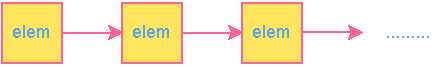
\includegraphics[scale=1]{./estáticos/node.pdf}
        \caption{Lista enlazada}
        \label{fig:my_label}
    \end{figure}
    \item Una lista será un puntero a un nodo.
    \item La lista vacía se implementa con el puntero null.
    \item Esta implementación permite tener la lista de elementos almacenada en lugares de la memoria no necesariamente contiguos.
    \item No existe límite teórico para almacenar elementos. En la práctica dicho límite será la cantidad de memoria.    
\end{itemize}

En resumen, la implementación de un TAD lista mediante punteros consiste en:
\begin{itemize}
    \item Definir un tipo nodo que contenga un elemento y un puntero al siguiente nodo.
    \item Definir un tipo lista que sea un puntero a un nodo.
    \item Implementar cada constructor y operación respetando los tipos especificados.
    \item Implementar la operación de destrucción liberando la memoria utilizada.
\end{itemize}

\textit{La implementación completa del TAD lista mediante punteros se encuentra en el solucionario.}

\section{TAD Contador}
Un problema interesante (y no del todo trivial) es el de controlar que una cierta expresión tiene balanceados sus paréntesis. Se quiere dar un algoritmo que tome una expresión (dada, por ejemplo, por un arreglo de caracteres) y devuelva verdadero si la expresión tiene sus paréntesis correctamente balanceados, y falso en caso contrario.
Este problema puede solucionarse con un algoritmo que recorre la expresión de izquierda a derecha y que utiliza un entero, que se inicializa en 0 y se incrementa cada vez que se encuentra un paréntesis que abre y se decrementa (chequeando previamente que dicho número no sea nulo) cada vez que se encuentra un paréntesis que cierra. Al analizar, sólo resta comprobar que dicho entero sea cero. Esta descripción debería alcanzar para darse uno cuenta de que no es en realidad un entero lo que hace falta, sino mucho menos. Un entero es un objeto que admite todas las operaciones aritméticas, acá sólo se necesita inicializar en 0, incrementar, decrementar y controlar si su valor es o no cero.

\subsection{Especificación}
Los \textbf{constructores} (en este caso inicial e incrementar) deben ser capaces de generar todos los valores posibles del TAD. En lo posible cada valor debe poder generarse de manera única. Intuitivamente, esto se cumple para inicial e incrementar: partiendo del valor inicial y tras sucesivos incrementos se puede alcanzar cualquier valor posible; y hay una única forma de alcanzar cada valor posible de esa manera.

Las demás \textbf{operaciones} quedan declaradas simplemente como tales. Las operaciones se definen con ecuaciones que deben cubrir todos los casos posibles, salvo los declarados que no pueden ocurrir, como en el caso de decrementar que no puede aplicarse a un contador que sea inicial (a pesar de que se podría defnir de manera obvia para ese caso). 
\begin{itemize}
    \item comprobar si su valor es el inicial
    \item decrementar si no lo es
\end{itemize}

\begin{codebox}{TAD Contador}
\begin{pascallike}
spec Counter where

constructors
    fun init() ret c : Counter
    {- crea un contador con valor inicial -}

    proc incr(in/out c : Counter)
    {- incrementa el valor del contador c -}

destroy
    proc destroy(in/out c : Counter)
    {- Libera memoria en caso que sea necesario. -}

operations
    fun is_init(c : Counter) ret b : bool
    {- Devuelve True si el contador c tiene el valor inicial -}

    {- PRE: not is_init(c) -}
    proc decr(in/out c : Counter)
    {- decrementa el valor del contador c -}
\end{pascallike}
\end{codebox}

\subsection{Implementación}

\begin{codebox}{Implementación del TAD Contador}
\begin{pascallike}
implement Counter where
type Counter = nat

proc init (out c: Counter)
    c:= 0
end proc

proc inc (in/out c: Counter)
    c:= c+1
end proc

fun is_init (c: Counter) ret b: bool
    b:= (c = 0)
end fun

{- PRE: not is_init(c) -}
proc dec (in/out c: Counter)
    c:= c-1
end proc

proc destroy (in/out c: Counter)
    skip
end proc
\end{pascallike}
\end{codebox}

\subsection{Algoritmo de balanceo de paréntesis}

\begin{codebox}{Algoritmo de balanceo de paréntesis}
\begin{pascallike}
fun matching_parenthesis (a: array[1..n] of char) ret b: bool
    var i: nat
    var c: Counter
    b:= true
    init(c)
    i:= 1
    do i $\leq$ n $\wedge$ b $\rightarrow$ if a[i] = '(' $\rightarrow$ inc(c)
                                    a[i] = ')' $\wedge$ is_init(c) $\rightarrow$ b:= false
                                    a[i] = ')' $\wedge$ $\neg$is_init(c) $\rightarrow$ dec(c)
                                    otherwise $\rightarrow$ skip
                                fi
                                i:= i+1
    od
    b:= b $\wedge$ is_init(c)
    destroy(c)
end fun
\end{pascallike}
\end{codebox}

\section{TAD Cola}

\subsection{Especificación}
\begin{itemize}
    \item \textbf{Nombre}: Cola
    \item \textbf{Constructores}:
    \begin{itemize}
        \item \texttt{empty()}: crea una cola vacía.
        \item \texttt{enqueue()}: agrega un elemento al final de la cola.
    \end{itemize}
    \item \textbf{Operaciones}:
    \begin{itemize}
        \item decidir si una cola es vacía,
        \item tomar el primer elemento,
        \item tirar el primer elemento,
        \item agregar un elemento al final,
        \item obtener la cantidad de elementos,
        \item copiar una cola en una nueva.
    \end{itemize}
\end{itemize}

\begin{codebox}{TAD Cola}
\begin{pascallike}
spec Queue of T where

constructors
    fun empty() ret q : Queue of T
    {- crea una cola vacia. -}

    proc enqueue(in e : T, in/out q : Queue of T)
    {- agrega el elemento e al final de la cola q. -}

destroy
    proc destroy(in/out q : Queue of T)
    {- Libera memoria en caso que sea necesario. -}

operations
    fun is_empty(q : Queue of T) ret b : bool
    {- Devuelve True si q es vacia. -}

    fun first(q : Queue of T) ret e : T
    {- Devuelve el primer elemento de la cola q -}

    {- PRE: not is_empty(q) -}
    proc dequeue(in/out q : Queue of T)
    {- Elimina el primer elemento de la cola q -}

    proc enqueue(in e : T, in/out q : Queue of T)
    {- agrega el elemento e al final de la cola q. -}

    fun length(q : Queue of T) ret n : nat
    {- Devuelve la cantidad de elementos de la cola q -}

    fun copy_queue(q1 : Queue of T) ret q2 : Queue of T
    {- Copia todos los elementos de q1 en la nueva cola q2 -}
\end{pascallike}
\end{codebox}

\subsection{Implementación}

\begin{codebox}{Implementación del TAD Cola}
\begin{pascallike}
implement Queue of T where
type Queue of T = record
    data: array[1..MAX] of T
    front: nat
    rear: nat
    size: nat
end record

proc empty (out q: Queue of T)
    q.front:= 1
    q.rear:= 0
    q.size:= 0
end proc

{- PRE: q.size < MAX -}
proc enqueue (in e: T, in/out q: Queue of T)
    q.rear:= (q.rear + 1) mod MAX
    q.data[q.rear]:= e
    q.size:= q.size + 1
end proc

fun is_empty (q: Queue of T) ret b: bool
    b:= (q.size = 0)
end fun

{- PRE: not is_empty(q) -}
proc dequeue (in/out q: Queue of T)
    q.front:= (q.front + 1) mod MAX
    q.size:= q.size - 1
end proc

fun first (q: Queue of T) ret e: T
    e:= q.data[q.front]
end fun

fun length (q: Queue of T) ret n: nat
    n:= q.size
end fun

fun copy_queue (q1: Queue of T) ret q2: Queue of T
    var i: nat
    q2.front:= 1
    q2.rear:= q1.size
    q2.size:= q1.size
    for i:= 1 to q1.size do
        q2.data[i]:= q1.data[(q1.front + i - 1) mod MAX]
    od
end fun

proc destroy (in/out q: Queue of T)
    skip
end proc
\end{pascallike}
\end{codebox}

\section{TAD Pila}

\subsection{Especificación}
\begin{itemize}
    \item \textbf{Nombre}: Pila
    \item \textbf{Constructores}:
    \begin{itemize}
        \item \texttt{empty()}: crea una pila vacía.
        \item \texttt{push()}: agrega un elemento al tope de la pila.
    \end{itemize}
    \item \textbf{Operaciones}:
    \begin{itemize}
        \item decidir si una pila es vacía,
        \item tomar el tope,
        \item tirar el tope,
        \item copiar una pila en una nueva.
    \end{itemize}
\end{itemize}

\begin{codebox}{TAD Pila}
\begin{pascallike}
spec Stack of T where

constructors
    fun empty() ret s : Stack of T
    {- crea una pila vacia. -}

    proc push(in e : T, in/out s : Stack of T)
    {- agrega el elemento e al tope de la pila s. -}

destroy
    proc destroy(in/out s : Stack of T)
    {- Libera memoria en caso que sea necesario. -}

operations
    fun is_empty(s : Stack of T) ret b : bool
    {- Devuelve True si s es vacia. -}

    fun top(s : Stack of T) ret e : T
    {- Devuelve el elemento del tope de la pila s -}

    {- PRE: not is_empty(s) -}
    proc pop(in/out s : Stack of T)
    {- Elimina el elemento del tope de la pila s -}

    fun copy_stack(s1 : Stack of T) ret s2 : Stack of T
    {- Copia todos los elementos de s1 en la nueva pila s2 -}
\end{pascallike}
\end{codebox}

\subsection{Implementación}

\begin{codebox}{Implementación del TAD Pila}
\begin{pascallike}
implement Stack of T where

type Node of T = tuple
                    elem : T
                    next : pointer to (Node of T)
                 end tuple

type Stack of T = pointer to (Node of T)

fun empty_stack() ret s: Stack of T
    s := null
end fun

proc push(in e: T, in/out s: Stack of T)
    var p: pointer to (Node of T)
    alloc(p)
    p->elem := e
    if s = null then
        s := p
    else
        p->next := s
        s := p
    fi
end proc 

fun is_empty_stack(s : Stack of T) ret b : Bool
    b := s = null
end fun

fun top(s : Stack of T) ret e : T
    e := s -> elem
end fun

proc pop (in/out s : Stack of T)
    var p: pointer to (Node of T)
    p := s
    s := s->next
    free(p)
end proc
\end{pascallike}
\end{codebox}

\begin{codebox}{Implementación del TAD Pila}
\begin{pascallike}
proc copy_stack(s1 : Stack of T) ret s2 : Stack of T
    var s10: pointer to (Node of T)
    var s20: pointer to (Node of T)
    var t : Node of T
    if is_empty_stack(s1) then
        s2 := empty_stack()
    else
        s10 := s1 
        s2->elem := s1->elem
        s2->next := null
        s20 := s2

    while s10 != null do
        alloc(t)
        t->elem := s10->elem
        t->next := null
        s10 := s10->next
        s20 := s20->next
    fi
end proc

proc destroy_stack(in/out s : Stack of T)
    var p: pointer to (Node of T)
    while s != null do
        p := s
        s := s->next
        free(p)
    od
end proc
\end{pascallike}
\end{codebox}

\section{TAD Multiset}

\subsection{Especificación}
\begin{itemize}
    \item \textbf{Nombre}: Multiconjunto
    \item \textbf{Constructores}:
    \begin{itemize}
        \item \texttt{empty()}: crea un multiconjunto vacío.
        \item \texttt{add\_elem()}: agrega un elemento al multiconjunto.
    \end{itemize}
    \item \textbf{Operaciones}:
    \begin{itemize}
        \item decidir si un multiconjunto es vacío,
        \item decidir si un elemento existe en el multiconjunto,
        \item devolver la cantidad de veces que un elemento aparece en el multiconjunto,
        \item eliminar un elemento del multiconjunto.
    \end{itemize}
\end{itemize}

\begin{codebox}{TAD Multiconjunto}
\begin{pascallike}
spec Multiset of T where

constructors
    fun empty() ret m : Multiset of T
    {- crea un multiconjunto vacio. -}

    proc add_elem(in e : T, in/out m : Multiset of T)
    {- agrega el elemento e al multiconjunto m. -}

destroy
    proc destroy(in/out m : Multiset of T)
    {- Libera memoria en caso que sea necesario. -}

operations
    fun is_empty(m : Multiset of T) ret b : bool
    {- Devuelve True si m es vacio. -}

    fun exists(in e : T, in m : Multiset of T) ret b : bool
    {- Devuelve True si e existe en el multiconjunto m. -}

    fun count(in e : T, in m : Multiset of T) ret n : nat
    {- Devuelve la cantidad de veces que e aparece en el multiconjunto m. -}

    {- PRE: exists(e,m) -}
    proc remove_elem(in e : T, in/out m : Multiset of T)
    {- Elimina una ocurrencia de e del multiconjunto m. -}
\end{pascallike}
\end{codebox}

\subsection{Implementación}

\begin{codebox}{Implementación del TAD Multiconjunto}
\begin{pascallike}
implement Multiset of T where

type par of T = tuple
                    elem: T
                    ocu: nat
                end tuple

type Multiset of T = List of par

fun empty_m() ret m: Multiset of T
    m := empty()
end fun

proc add_elem(in e: T, in/out m: Multiset of T)
    var p: par of T
    var n: Multiset of T
    p.elem := e
    p.ocu := 1
    if is_empty(m) then
        addl(p, m)
    else
        n := copy_list(m)
        do not is_empty(n) -> 
            if (head(n).elem = e) then
                head(n).ocu := head(n)->ocu + 1
            fi
            tail(n)
        od
        addl(p, m)
    fi
end proc

proc destroy_m(in/out m: Multiset of T)
    destroy(m)
end proc

fun exits(m: Multiset of T, e: T) ret b: bool
    var n: Multiset of T
    var tmp: par of T
    b := false
    n := copy_list(m)
    do not is_empty(n) ->
        tmp := head(n)
        if (tmp.elem = e) then
            b := true
        fi
        tail(n)
    od
end fun
\end{pascallike}
\end{codebox}

\begin{codebox}{Implementación del TAD Multiconjunto}
\begin{pascallike}
fun hm_ocu(m: Multiset of T, e: T) ret k: nat
    var n: Multiset of T
    var tmp: par of T
    k := 0
    n := copy_list(m)
    do not is_empty(n) ->
        tmp := head(n)
        if (tmp.elem = e) then
            k := k+1
        fi
        tail(n)
    od
end fun

fun del_ocu(in/out m: Multiset of T, e: T)
    var n,o: Multiset of T
    n := copy_list(m)
    o := copy_list(m)
    var index : nat
    var tmp: par of T
    index := 1
    do not is_empty(n) ->
        tmp := head(n)
        if(tmp.elem = e) 
            destroy(n)
        fi
        else index := index +1
        tail(n)
    od
    m := concat(take(o,index-1), drop(o,index+1))
end fun
\end{pascallike}
\end{codebox}

\subsection{Ejemplo de uso}

\begin{codebox}{Ejemplo de uso del TAD Multiconjunto}
\footnotesize Devolver elementos pares del multiconjunto
\tcblower
\begin{pascallike}
fun mul_pares(a : array[1..N] of nat) ret m: Multiset of T
    {-pongo los pares en el multiconjunto-}
    m := empty_m()
    for i := 1 to N do
        if a[i] mod 2 = 0 then
            add_elem(a[i], m)
        fi
    od
end fun
\end{pascallike}
\end{codebox}

\section{TAD Árbol Binario}

\subsection{Especificación}
\begin{itemize}
    \item \textbf{Nombre}: Árbol Binario
    \item \textbf{Constructores}:
    \begin{itemize}
        \item \texttt{empty()}: crea un árbol binario vacío.
        \item \texttt{node(tl, e, tr)}: crea el nodo con elemento e y subárboles izquierdo y derecho tl y tr. 
    \end{itemize}
    \item \textbf{Operaciones}:
    \begin{itemize}
        \item decidir si un árbol binario es vacío,
        \item devuelve el elemento que se encuentra en la raíz,
        \item devuelve el subárbol izquierdo,
        \item devuelve el subárbol derecho,
        \item devuelve la distancia entre la raíz y la hoja más lejana,
        \item decidir si p es un camino válido en el árbol,
        \item devuelve el subarbol que contiene a p,
        \item devuelve el elemento que se encuentra en la posición p.
    \end{itemize}
\end{itemize}

\begin{codebox}{TAD Árbol Binario}
\begin{pascallike}
spec BinaryTree of T where

constructors
    fun empty() ret t : BinaryTree of T
    {- crea un arbol binario vacio. -}

    fun node(in tl : BinaryTree of T, in e : T, in tr : BinaryTree of T) 
    ret t : BinaryTree of T
    {- crea un nodo con elemento e y subarboles izquierdo y derecho tl y tr. -}

destroy
    proc destroy(in/out t : BinaryTree of T)
    {- Libera memoria en caso que sea necesario. -}

operations
    fun is_empty(t : BinaryTree of T) ret b : bool
    {- Devuelve True si t es vacio. -}

    fun root(t : BinaryTree of T) ret e : T
    {- Devuelve el elemento de la raiz del arbol t -}
    {- PRE: not is_empty(t) -}

    fun left(t : BinaryTree of T) ret tl : BinaryTree of T
    {- Devuelve el subarbol izquierdo de t -}

    fun right(t : BinaryTree of T) ret tr : BinaryTree of T
    {- Devuelve el subarbol derecho de t -}
\end{pascallike}
\end{codebox}
\begin{codebox}{TAD Árbol Binario}
\begin{pascallike}
    fun height(t : BinaryTree of T) ret h : nat
    {- Devuelve la distancia entre la raiz y la hoja mas lejana -}

    fun is_path(t : BinaryTree of T, in p : List of nat) ret b : bool
    {- Devuelve True si p es un camino valido en el arbol t -}

    fun subtree(t : BinaryTree of T, in p : List of nat) ret st : BinaryTree of T
    {- Devuelve el subarbol que contiene a p -}

    fun element(t : BinaryTree of T, in p : List of nat) ret e : T
    {- Devuelve el elemento que se encuentra en la posicion p -}
\end{pascallike}
\end{codebox}

\subsection{Implementación}

\begin{codebox}{Implementación del TAD Árbol Binario}
\begin{pascallike}
implement BinaryTree of T where

type Node of T = tuple
                    left : pointer to (Node of T)
                    value : T
                    right : pointer to (Node of T)
                 end tuple

type BinaryTree of T = pointer to (Node of T)

fun empty() ret t : BinaryTree of T
    t := null
end fun

fun node(in tl : BinaryTree of T, in e : T, in tr : BinaryTree of T)
ret t : BinaryTree of T
    var p: pointer to (Node of T)
    alloc(p)
    p->left := tl
    p->value := e
    p->right := tr
    t := p
end fun

fun is_empty(t : BinaryTree of T) ret b : bool
    b := t = null
end fun

fun root(t : BinaryTree of T) ret e : T
    e := t->value
end fun

fun left(t : BinaryTree of T) ret tl : BinaryTree of T
    tl := t->left
end fun

fun right(t : BinaryTree of T) ret tr : BinaryTree of T
    tr := t->right
end fun
\end{pascallike}
\end{codebox}
\begin{codebox}{Implementación del TAD Árbol Binario}
\begin{pascallike}
fun height(t : BinaryTree of T) ret h : nat
    var hl, hr: nat
    if t = null then
        h := 0
    else
        hl := height(t->left)
        hr := height(t->right)
        if hl > hr then
            h := hl + 1
        else
            h := hr + 1
        fi
    fi
end fun

fun is_path(t : BinaryTree of T, in p : List of nat) ret b : bool
    var n: nat
    var tl: BinaryTree of T
    b := true
    n := length(p)
    tl := t
    for i:= 1 to n do
        if p[i] = 0 then
            tl := left(tl)
        else
            tl := right(tl)
        fi
        if tl = null then
            b := false
        fi
    od
end fun

fun subtree(t : BinaryTree of T, in p : List of nat) ret st : BinaryTree of T
    var n: nat
    var tl: BinaryTree of T
    n := length(p)
    tl := t
    for i:= 1 to n do
        if p[i] = 0 then
            tl := left(tl)
        else
            tl := right(tl)
        fi
    od
    st := tl
end fun

fun element(t : BinaryTree of T, in p : List of nat) ret e : T
    var n: nat
    var tl: BinaryTree of T
    n := length(p)
    tl := t
    for i:= 1 to n do
        if p[i] = 0 then
            tl := left(tl)
        else
            tl := right(tl)
        fi
    od
    e := root(tl)
end fun
\end{pascallike}
\end{codebox}
\begin{codebox}{Implementación del TAD Árbol Binario}
\begin{pascallike}
proc destroy(in/out t : BinaryTree of T)
    var tl, tr: BinaryTree of T
    if t != null then
        tl := left(t)
        tr := right(t)
        destroy(tl)
        destroy(tr)
        free(t)
    fi
end proc

\end{pascallike}
\end{codebox}